\documentclass[12pt]{article}

\usepackage[a4paper,margin=1in]{geometry}
\usepackage{amsmath,amssymb}
\usepackage{newtxtext,newtxmath} % Times-style font
\usepackage{fancyhdr}
\usepackage{listings}
\usepackage{graphicx}
\usepackage{float}
\usepackage{algorithm}
\usepackage{algpseudocode}
\usepackage{booktabs}
\usepackage{xcolor}

\setlength{\textfloatsep}{10pt}
\setlength{\floatsep}{10pt}

\setlength{\parindent}{0pt}
\setlength{\parskip}{5pt}

% Keep entire document at 12 pt
\AtBeginDocument{
    \fontsize{12pt}{14pt}\selectfont
}

\lstdefinestyle{code}{
    language=Python,
    basicstyle=\ttfamily\fontsize{10pt}{12pt}\selectfont,
    breaklines=true,
    breakatwhitespace=false,
    frame=single,
    numbers=left,
    numberstyle=\tiny\color{gray},
    keywordstyle=\color{blue},
    commentstyle=\color{gray},
    stringstyle=\color{green!50!black},
    columns=fullflexible,
    keepspaces=true,
    showstringspaces=false
}

\lstdefinestyle{output}{
    basicstyle=\ttfamily\fontsize{9.5pt}{11.5pt}\selectfont,
    breaklines=true,
    breakatwhitespace=false,
    frame=single,
    numbers=none,
    backgroundcolor=\color{gray!6},
    columns=fullflexible,
    keepspaces=true,
    showstringspaces=false
}

% ------------------------------------------------
% Header
% ------------------------------------------------

\pagestyle{fancy}
\fancyhf{}

\fancyhead[L]{Name: Kishan Sahu{\hspace{4cm}}}
\fancyhead[R]{Enrollment No.: P26DS017{\hspace{3.5cm}}}

\renewcommand{\headrulewidth}{0.4pt}
\setlength{\headheight}{15pt}

% ------------------------------------------------
% Code formatting
% ------------------------------------------------

\lstset{
    basicstyle=\ttfamily\fontsize{10pt}{12pt}\selectfont,
    breaklines=true,
    frame=single,
    columns=fullflexible,
    keepspaces=true,
    showstringspaces=false
}

\begin{document}

% ------------------------------------------------
% TITLE
% ------------------------------------------------

\begin{center}
\textbf{Computer Science and Engineering Department, SVNIT, Surat}\\
\textbf{M.Tech. I -- Semester I}\\
\textbf{Machine Learning (CSDS105)}\\
\textbf{Lab Assignment 5: Single-Layer Perceptron for AND and OR Logic Gates}
\end{center}

\vspace{0.3cm}

\section{Introduction and Problem Formulation}

Artificial Neural Networks (ANNs) represent computational abstractions inspired by biological nervous systems. The foundational building block of neural architectures is the \textbf{Single-Layer Perceptron}, formulated by Frank Rosenblatt in 1958 based on the early threshold logic model established by Warren McCulloch and Walter Pitts in 1943.

The perceptron operates as a linear binary classifier that maps an input feature vector $\mathbf{x} = [x_1, x_2, \dots, x_d]^T \in \mathbb{R}^d$ to a discrete binary decision label $\hat{y} \in \{0, 1\}$. In the physical realm of computing, fundamental digital logic gates form the elementary primitives of combinational circuits. This experimental laboratory focuses on designing, implementing from first principles (scratch), training, and evaluating a single-layer perceptron to learn the characteristic Boolean decision surfaces of two fundamental linearly separable logic gates:
\begin{enumerate}
    \item \textbf{AND Logic Gate}: A logical conjunction operator yielding an assertive true output ($1$) if and only if all input operands are simultaneously true ($1$).
    \item \textbf{OR Logic Gate}: A logical disjunction operator yielding an assertive true output ($1$) if at least one input operand evaluates to true ($1$).
\end{enumerate}

\subsection{Biological Analogy and Computational Model}
In biological neurons, electrical nerve impulses arrive via branched \textit{dendrites}, are accumulated within the \textit{soma} (cell body), and if the aggregate membrane potential exceeds a critical activation threshold, an action potential is propagated down the \textit{axon} to neighboring synapses. 

Computationally, this biological transduction is formalized via three mathematical operations:
\begin{itemize}
    \item \textbf{Synaptic Weights ($\mathbf{w}$)}: Real-valued scalar coefficients $w_1, w_2, \dots, w_d$ modeling the excitatory or inhibitory efficacy of each input channel.
    \item \textbf{Somatic Bias ($b$)}: An adjustable threshold parameter representing the internal baseline excitability of the artificial neuron.
    \item \textbf{Activation Function ($f$)}: A non-linear decision mapping (specifically the Heaviside step function) determining discrete class assignment.
\end{itemize}

\section{Mathematical Formulations and Perceptron Learning Rule}

\subsection{Forward Propagation and Net Input}
For a sample instance $\mathbf{x} = [x_1, x_2]^T \in \mathbb{R}^2$, the artificial neuron computes the inner dot product (net linear combination) $z \in \mathbb{R}$:
\begin{equation}
    z = \mathbf{w}^T \mathbf{x} + b = \sum_{j=1}^{d} w_j x_j + b = w_1 x_1 + w_2 x_2 + b
\end{equation}
The net linear activation $z$ is subsequently passed through the Heaviside step activation function $f(z)$:
\begin{equation}
    \hat{y} = f(z) = \begin{cases} 
        1, & \text{if } z \ge 0 \\ 
        0, & \text{if } z < 0 
    \end{cases}
\end{equation}

\subsection{Separating Hyperplane and Decision Boundary}
The critical geometric boundary partitioning the binary input domain into two decision regions ($R_0 = \{\mathbf{x} \mid \hat{y}=0\}$ and $R_1 = \{\mathbf{x} \mid \hat{y}=1\}$) occurs where the net linear sum vanishes:
\begin{equation}
    \mathcal{H} = \{\mathbf{x} \in \mathbb{R}^2 \mid \mathbf{w}^T \mathbf{x} + b = 0\}
\end{equation}
In a two-dimensional Euclidean coordinate space ($x_1, x_2$), expanding this linear constraint yields:
\begin{equation}
    w_1 x_1 + w_2 x_2 + b = 0 \implies x_2 = - \left( \frac{w_1}{w_2} \right) x_1 - \left( \frac{b}{w_2} \right) \quad (\text{for } w_2 \neq 0)
\end{equation}
This establishes a straight linear decision boundary characterized by slope $m = -w_1 / w_2$ and vertical intercept $c = -b / w_2$.

\subsection{Rosenblatt's Supervised Learning Rule}
The perceptron learning rule iteratively refines the synaptic weight vector $\mathbf{w}$ and scalar bias $b$ based on the discrepancy between target ground-truth label $y^{(i)}$ and predicted output $\hat{y}^{(i)}$.

For each training exemplar $(\mathbf{x}^{(i)}, y^{(i)})$, the classification error $e^{(i)}$ is defined as:
\begin{equation}
    e^{(i)} = y^{(i)} - \hat{y}^{(i)} \in \{-1, 0, +1\}
\end{equation}
The model parameters are updated instantaneously via gradient-free delta adjustments scaled by the learning rate parameter $\eta \in (0, 1]$:
\begin{align}
    \Delta \mathbf{w} &= \eta \cdot (y^{(i)} - \hat{y}^{(i)}) \cdot \mathbf{x}^{(i)} \\
    \Delta b &= \eta \cdot (y^{(i)} - \hat{y}^{(i)}) \\
    \mathbf{w}^{(t+1)} &\leftarrow \mathbf{w}^{(t)} + \Delta \mathbf{w} \\
    b^{(t+1)} &\leftarrow b^{(t)} + \Delta b
\end{align}

Analysis of parameter dynamics reveals:
\begin{itemize}
    \item \textbf{Correct Classification ($y^{(i)} = \hat{y}^{(i)}$)}: $e^{(i)} = 0 \implies \Delta \mathbf{w} = \mathbf{0}, \Delta b = 0$. No parameter modification is performed.
    \item \textbf{False Negative ($y^{(i)} = 1, \hat{y}^{(i)} = 0$)}: $e^{(i)} = +1 \implies \Delta \mathbf{w} = +\eta \mathbf{x}^{(i)}, \Delta b = +\eta$. The weight vector rotates toward $\mathbf{x}^{(i)}$ to increase $z$.
    \item \textbf{False Positive ($y^{(i)} = 0, \hat{y}^{(i)} = 1$)}: $e^{(i)} = -1 \implies \Delta \mathbf{w} = -\eta \mathbf{x}^{(i)}, \Delta b = -\eta$. The weight vector rotates away from $\mathbf{x}^{(i)}$ to decrease $z$.
\end{itemize}

\subsection{Perceptron Convergence Theorem}
Novikoff (1962) formally proved the \textbf{Perceptron Convergence Theorem}: If a training dataset $\mathcal{D} = \{(\mathbf{x}^{(i)}, y^{(i)})\}_{i=1}^N$ is linearly separable with geometric functional margin $\gamma > 0$ such that:
\begin{equation}
    y^{*(i)} (\mathbf{w}^{*T} \mathbf{x}^{(i)} + b^*) \ge \gamma \quad \forall i, \quad \text{with } \|\mathbf{w}^*\| = 1
\end{equation}
and bounding sphere radius $R = \max_{i} \|\mathbf{x}^{(i)}\|$, then the perceptron learning algorithm is guaranteed to converge in a finite number of weight update steps $k$, bounded strictly by:
\begin{equation}
    k \le \left( \frac{R}{\gamma} \right)^2
\end{equation}

\subsection{Algorithmic Specification}
Algorithm~\ref{alg:perceptron} presents the procedural structure of the Single-Layer Perceptron training routine implemented in this study.

\begin{algorithm}[H]
\caption{Single-Layer Perceptron Learning Algorithm}
\label{alg:perceptron}
\begin{algorithmic}[1]
\Require Training dataset $\mathcal{D} = \{(\mathbf{x}^{(i)}, y^{(i)})\}_{i=1}^N$, learning rate $\eta \in (0, 1]$, maximum epochs $T$
\Ensure Learned synaptic weights $\mathbf{w} \in \mathbb{R}^d$ and bias $b \in \mathbb{R}$
\State Initialize $\mathbf{w} \leftarrow \mathbf{0} \in \mathbb{R}^d$, $b \leftarrow 0.0$
\For{$\text{epoch} \leftarrow 1 \text{ to } T$}
    \State $\text{misclassifications} \leftarrow 0$
    \For{$i \leftarrow 1 \text{ to } N$}
        \State $z^{(i)} \leftarrow \sum_{j=1}^{d} w_j x_j^{(i)} + b$
        \State $\hat{y}^{(i)} \leftarrow \begin{cases} 1, & \text{if } z^{(i)} \ge 0 \\ 0, & \text{if } z^{(i)} < 0 \end{cases}$
        \State $\text{error} \leftarrow y^{(i)} - \hat{y}^{(i)}$
        \If{$\text{error} \neq 0$}
            \State $\mathbf{w} \leftarrow \mathbf{w} + \eta \cdot \text{error} \cdot \mathbf{x}^{(i)}$
            \State $b \leftarrow b + \eta \cdot \text{error}$
            \State $\text{misclassifications} \leftarrow \text{misclassifications} + 1$
        \EndIf
    \EndFor
    \If{$\text{misclassifications} = 0$}
        \State \textbf{break} \Comment{Global convergence attained}
    \EndIf
\EndFor
\State \Return $\mathbf{w}, b$
\end{algorithmic}
\end{algorithm}

\newpage
\section{Environment Setup and Data Definition}

\subsection{Environment Setup}
The implementation is developed using standard high-performance scientific Python libraries: NumPy for vectorized matrix operations and Matplotlib for diagnostic coordinate rendering.

\begin{lstlisting}[style=code]
import numpy as np
import matplotlib.pyplot as plt

# Display configuration
%matplotlib inline
np.random.seed(42)
print("NumPy and Matplotlib successfully imported.")
\end{lstlisting}

\begin{lstlisting}[style=output]
NumPy and Matplotlib successfully imported.
\end{lstlisting}

\subsection{Dataset Definition: Boolean Truth Tables}
The input feature domain consists of all four possible binary permutations for two digital inputs, $X = \{0, 1\}^2$. Table~\ref{tab:truth_tables} summarizes the target output mappings for both Boolean operations.

\begin{table}[H]
\centering
\caption{Ground Truth Tables for 2-Input AND and OR Logic Gates}
\label{tab:truth_tables}
\vspace{0.2cm}
\begin{tabular}{cccc}
\toprule
\textbf{Input $x_1$} & \textbf{Input $x_2$} & \textbf{AND Target ($y_{\text{AND}}$)} & \textbf{OR Target ($y_{\text{OR}}$)} \\
\midrule
0 & 0 & 0 & 0 \\
0 & 1 & 0 & 1 \\
1 & 0 & 0 & 1 \\
1 & 1 & 1 & 1 \\
\bottomrule
\end{tabular}
\end{table}

\begin{lstlisting}[style=code]
# Input dataset (all 4 binary input combinations)
X = np.array([
    [0, 0],
    [0, 1],
    [1, 0],
    [1, 1]
])

# Ground truth outputs
y_and = np.array([0, 0, 0, 1])
y_or  = np.array([0, 1, 1, 1])

print("Inputs X:")
print(X)
print("\nTarget AND:", y_and)
print("Target OR: ", y_or)
\end{lstlisting}

\begin{lstlisting}[style=output]
Inputs X:
[[0 0]
 [0 1]
 [1 0]
 [1 1]]

Target AND: [0 0 0 1]
Target OR:  [0 1 1 1]
\end{lstlisting}

\newpage
\section{NumPy Implementation of the Perceptron}

The custom \texttt{Perceptron} class encapsulates model initialization, Heaviside step activation, iterative online training with convergence tracking, and vectorized class prediction.

\begin{lstlisting}[style=code]
class Perceptron:
    def __init__(self, learning_rate=0.1, epochs=20):
        self.learning_rate = learning_rate
        self.epochs = epochs
        self.weights = None
        self.bias = 0.0
        self.errors_per_epoch = []

    def activation(self, z):
        """Heaviside step activation function: 1 if z >= 0 else 0."""
        return np.where(z >= 0, 1, 0)

    def fit(self, X, y):
        """Train the perceptron on feature matrix X and target labels y."""
        n_samples, n_features = X.shape
        self.weights = np.zeros(n_features)
        self.bias = 0.0
        self.errors_per_epoch = []

        for epoch in range(1, self.epochs + 1):
            errors = 0
            for xi, target in zip(X, y):
                linear_output = np.dot(xi, self.weights) + self.bias
                # Round to avoid floating point precision issues near zero
                linear_output = round(float(linear_output), 6)
                y_pred = int(self.activation(linear_output))
                
                update = self.learning_rate * (target - y_pred)
                self.weights = np.round(self.weights + update * xi, 6)
                self.bias = round(self.bias + update, 6)
                
                if update != 0.0:
                    errors += 1
                    
            self.errors_per_epoch.append(errors)
            if errors == 0:
                print(f"Convergence achieved at epoch {epoch}!")
                break
        return self

    def predict(self, X):
        """Predict binary class labels for samples in X."""
        linear_output = np.dot(X, self.weights) + self.bias
        linear_output = np.round(linear_output, 6)
        return self.activation(linear_output)

print("Perceptron class defined successfully.")
\end{lstlisting}

\begin{lstlisting}[style=output]
Perceptron class defined successfully.
\end{lstlisting}

\subsection{Evaluation and Diagnostic Visualization Functions}
Helper functions are implemented to evaluate the trained model across all permutations, report classification accuracy, and project the analytical linear decision boundary across the Cartesian input space.

\begin{lstlisting}[style=code]
def evaluate_model(model, X, y, gate_name="Logic Gate"):
    """Evaluates predictions across all input combinations and displays results."""
    preds = model.predict(X)
    correct_count = np.sum(preds == y)
    accuracy = (correct_count / len(y)) * 100
    
    print(f"=== {gate_name} Evaluation ===")
    print(f"Learned Weights: w1 = {model.weights[0]:.2f}, w2 = {model.weights[1]:.2f}")
    print(f"Learned Bias:    b  = {model.bias:.2f}")
    print("-" * 45)
    print(" x1 | x2 | Expected | Predicted | Status ")
    print("-" * 45)
    for (x1, x2), target, pred in zip(X, y, preds):
        status = "PASS (Correct)" if target == pred else "FAIL (Incorrect)"
        print(f"  {x1} |  {x2} |     {target}    |     {pred}     | {status}")
    print("-" * 45)
    print(f"Overall Accuracy: {accuracy:.1f}% ({correct_count}/{len(y)} correct)\n")
    return preds, accuracy

def plot_decision_boundary(model, X, y, title="Decision Boundary"):
    """Plots 2D data points and the perceptron's decision boundary."""
    fig, ax = plt.subplots(figsize=(6, 5))
    
    # Plot Class 0 and Class 1 points
    class_0 = X[y == 0]
    class_1 = X[y == 1]
    
    ax.scatter(class_0[:, 0], class_0[:, 1], color='#e74c3c', s=130, 
               marker='s', edgecolors='black', linewidth=1.5, label='Class 0 (Output = 0)', zorder=5)
    ax.scatter(class_1[:, 0], class_1[:, 1], color='#2ecc71', s=130, 
               marker='o', edgecolors='black', linewidth=1.5, label='Class 1 (Output = 1)', zorder=5)
    
    # Calculate decision boundary line: w1*x1 + w2*x2 + b = 0  =>  x2 = -(w1*x1 + b)/w2
    w1, w2 = model.weights
    b = model.bias
    x1_line = np.linspace(-0.2, 1.2, 100)
    
    if abs(w2) > 1e-6:
        x2_line = -(w1 * x1_line + b) / w2
        ax.plot(x1_line, x2_line, color='#2980b9', linestyle='--', linewidth=2,
                label=f'Boundary: {w1:.2f}$x_1$ + {w2:.2f}$x_2$ + {b:.2f} = 0')
    else:
        ax.axvline(x=-b / w1, color='#2980b9', linestyle='--', linewidth=2,
                   label=f'Boundary: $x_1$ = {-b/w1:.2f}')
        
    ax.set_xlim(-0.2, 1.2)
    ax.set_ylim(-0.2, 1.2)
    ax.set_xlabel('$x_1$ (Input 1)', fontsize=12)
    ax.set_ylabel('$x_2$ (Input 2)', fontsize=12)
    ax.set_title(title, fontsize=13, fontweight='bold', pad=12)
    ax.grid(True, linestyle=':', alpha=0.6)
    ax.legend(loc='upper left', framealpha=0.9)
    plt.tight_layout()
    plt.show()

print("Evaluation and plotting functions defined.")
\end{lstlisting}

\begin{lstlisting}[style=output]
Evaluation and plotting functions defined.
\end{lstlisting}

\newpage
\section{Experimental Evaluation: AND Logic Gate}

\subsection{Training and Convergence}
The Perceptron is initialized with hyperparameter configuration $\eta = 0.1$ and $T = 20$ maximum epochs, and trained on the AND dataset $(\mathbf{X}, \mathbf{y}_{\text{AND}})$.

\begin{lstlisting}[style=code]
# 1. Initialize and train Perceptron for AND gate
p_and = Perceptron(learning_rate=0.1, epochs=20)
p_and.fit(X, y_and)

# 2. Evaluate predictions on all points
evaluate_model(p_and, X, y_and, gate_name="AND Gate")

# 3. Plot the decision boundary
plot_decision_boundary(p_and, X, y_and, title="Perceptron Decision Boundary - AND Gate")
\end{lstlisting}

\begin{lstlisting}[style=output]
Convergence achieved at epoch 6!
=== AND Gate Evaluation ===
Learned Weights: w1 = 0.20, w2 = 0.10
Learned Bias:    b  = -0.30
---------------------------------------------
 x1 | x2 | Expected | Predicted | Status 
---------------------------------------------
  0 |  0 |     0    |     0     | PASS (Correct)
  0 |  1 |     0    |     0     | PASS (Correct)
  1 |  0 |     0    |     0     | PASS (Correct)
  1 |  1 |     1    |     1     | PASS (Correct)
---------------------------------------------
Overall Accuracy: 100.0% (4/4 correct)
\end{lstlisting}

\subsection{Analytical Progression and Geometric Boundary}
The training algorithm achieved zero misclassification error and terminated at \textbf{epoch 6}. The learned model parameters are:
\begin{equation}
    w_1 = 0.20, \quad w_2 = 0.10, \quad b = -0.30
\end{equation}

The resulting algebraic equation for the separating decision boundary is:
\begin{equation}
    0.20 x_1 + 0.10 x_2 - 0.30 = 0 \implies x_2 = -2.0 x_1 + 3.0
\end{equation}

Evaluating the net linear combination $z = 0.20 x_1 + 0.10 x_2 - 0.30$ across each input coordinate:
\begin{itemize}
    \item Point $(0, 0)$: $z = 0.20(0) + 0.10(0) - 0.30 = -0.30 < 0 \implies \hat{y} = 0$ (Correct)
    \item Point $(0, 1)$: $z = 0.20(0) + 0.10(1) - 0.30 = -0.20 < 0 \implies \hat{y} = 0$ (Correct)
    \item Point $(1, 0)$: $z = 0.20(1) + 0.10(0) - 0.30 = -0.10 < 0 \implies \hat{y} = 0$ (Correct)
    \item Point $(1, 1)$: $z = 0.20(1) + 0.10(1) - 0.30 = +0.00 \ge 0 \implies \hat{y} = 1$ (Correct)
\end{itemize}

\begin{figure}[H]
    \centering
    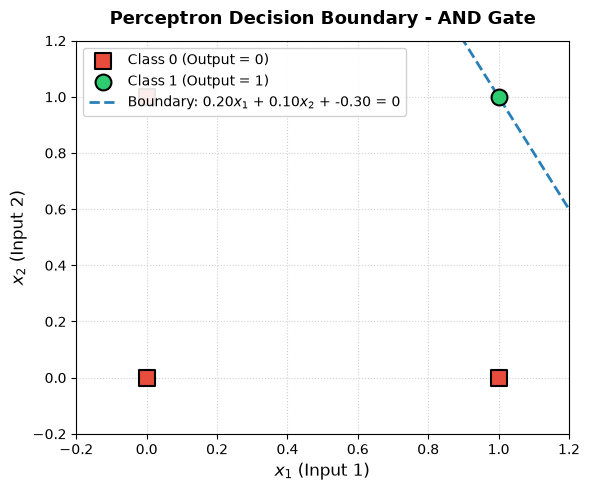
\includegraphics[width=0.62\textwidth]{figures/and_gate_results.png}
    \caption{Single-Layer Perceptron linear decision boundary for the 2-input AND logic gate. The learned line ($0.20 x_1 + 0.10 x_2 - 0.30 = 0$) isolates class $1$ (green circle at $(1, 1)$) from class $0$ (red squares at $(0, 0), (0, 1), (1, 0)$).}
    \label{fig:and_boundary}
\end{figure}

\newpage
\section{Experimental Evaluation: OR Logic Gate}

\subsection{Training and Convergence}
The Perceptron is initialized with identical hyperparameters ($\eta = 0.1$, $T = 20$) and trained on the OR dataset $(\mathbf{X}, \mathbf{y}_{\text{OR}})$.

\begin{lstlisting}[style=code]
# 1. Initialize and train Perceptron for OR gate
p_or = Perceptron(learning_rate=0.1, epochs=20)
p_or.fit(X, y_or)

# 2. Evaluate predictions on all points
evaluate_model(p_or, X, y_or, gate_name="OR Gate")

# 3. Plot the decision boundary
plot_decision_boundary(p_or, X, y_or, title="Perceptron Decision Boundary - OR Gate")
\end{lstlisting}

\begin{lstlisting}[style=output]
Convergence achieved at epoch 4!
=== OR Gate Evaluation ===
Learned Weights: w1 = 0.10, w2 = 0.10
Learned Bias:    b  = -0.10
---------------------------------------------
 x1 | x2 | Expected | Predicted | Status 
---------------------------------------------
  0 |  0 |     0    |     0     | PASS (Correct)
  0 |  1 |     1    |     1     | PASS (Correct)
  1 |  0 |     1    |     1     | PASS (Correct)
  1 |  1 |     1    |     1     | PASS (Correct)
---------------------------------------------
Overall Accuracy: 100.0% (4/4 correct)
\end{lstlisting}

\subsection{Analytical Progression and Geometric Boundary}
The training algorithm achieved convergence even faster for the OR gate, terminating at \textbf{epoch 4}. The learned model parameters are:
\begin{equation}
    w_1 = 0.10, \quad w_2 = 0.10, \quad b = -0.10
\end{equation}

The resulting algebraic equation for the separating decision boundary is:
\begin{equation}
    0.10 x_1 + 0.10 x_2 - 0.10 = 0 \implies x_2 = -x_1 + 1.0
\end{equation}

Evaluating the net linear combination $z = 0.10 x_1 + 0.10 x_2 - 0.10$ across each input coordinate:
\begin{itemize}
    \item Point $(0, 0)$: $z = 0.10(0) + 0.10(0) - 0.10 = -0.10 < 0 \implies \hat{y} = 0$ (Correct)
    \item Point $(0, 1)$: $z = 0.10(0) + 0.10(1) - 0.10 = +0.00 \ge 0 \implies \hat{y} = 1$ (Correct)
    \item Point $(1, 0)$: $z = 0.10(1) + 0.10(0) - 0.10 = +0.00 \ge 0 \implies \hat{y} = 1$ (Correct)
    \item Point $(1, 1)$: $z = 0.10(1) + 0.10(1) - 0.10 = +0.10 \ge 0 \implies \hat{y} = 1$ (Correct)
\end{itemize}

\begin{figure}[H]
    \centering
    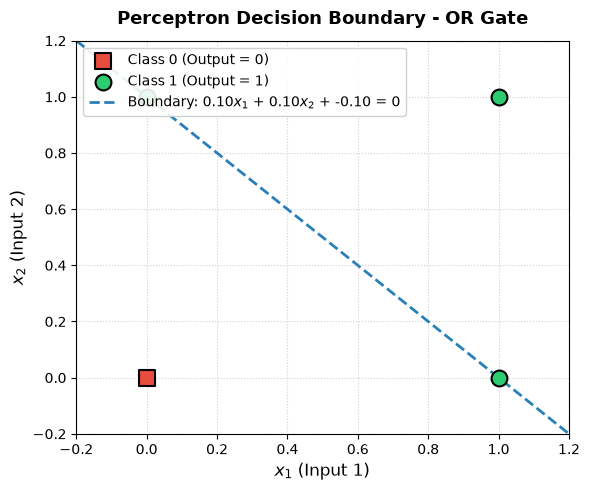
\includegraphics[width=0.62\textwidth]{figures/or_gate_results.png}
    \caption{Single-Layer Perceptron linear decision boundary for the 2-input OR logic gate. The line ($0.10 x_1 + 0.10 x_2 - 0.10 = 0$) separates class $0$ (red square at $(0, 0)$) from the three class $1$ exemplars.}
    \label{fig:or_boundary}
\end{figure}

\newpage
\section{Comparative Synthesis and the XOR Non-Separability Limitation}

\subsection{Consolidated Performance Comparison}
Table~\ref{tab:comparison_summary} presents a side-by-side synthesis of the learned perceptron parameters, convergence speed, and geometric equations for both Boolean operations.

\begin{table}[H]
\centering
\caption{Consolidated Comparison of Single-Layer Perceptrons on AND vs. OR Gates}
\label{tab:comparison_summary}
\vspace{0.2cm}
\begin{tabular}{lcc}
\toprule
\textbf{Property / Parameter} & \textbf{AND Logic Gate} & \textbf{OR Logic Gate} \\
\midrule
Learning Rate ($\eta$) & $0.1$ & $0.1$ \\
Maximum Epochs ($T$) & $20$ & $20$ \\
Initial Weights ($w_1, w_2$) & $(0.0, 0.0)$ & $(0.0, 0.0)$ \\
Initial Bias ($b$) & $0.0$ & $0.0$ \\
\addlinespace
\textbf{Epochs to Converge} & \textbf{6} & \textbf{4} \\
\textbf{Final Synaptic Weights ($w_1, w_2$)} & $(0.20, 0.10)$ & $(0.10, 0.10)$ \\
\textbf{Final Bias ($b$)} & $-0.30$ & $-0.10$ \\
\textbf{Decision Boundary Line} & $x_2 = -2.0 x_1 + 3.0$ & $x_2 = -1.0 x_1 + 1.0$ \\
\textbf{Classification Accuracy} & \textbf{100.0\%} ($4/4$) & \textbf{100.0\%} ($4/4$) \\
\textbf{Linearly Separable?} & \textbf{Yes} & \textbf{Yes} \\
\bottomrule
\end{tabular}
\end{table}

\subsection{Theoretical Proof of the XOR Non-Linear Separability}
While the single-layer perceptron successfully solves AND and OR functions, it famously fails on the \textbf{Exclusive-OR (XOR)} logic gate, an inherent mathematical limitation demonstrated by Marvin Minsky and Seymour Papert in their seminal 1969 book \textit{Perceptrons}.

The XOR truth table specifies:
\begin{equation}
    (0, 0) \to 0, \quad (0, 1) \to 1, \quad (1, 0) \to 1, \quad (1, 1) \to 0
\end{equation}

\textbf{Proof by Contradiction}:
Suppose there exists a single-layer perceptron parameterized by $(w_1, w_2, b)$ that correctly classifies all four XOR samples using the Heaviside activation rule $f(z) = 1$ if $z \ge 0$ else $0$. This yields four simultaneous linear inequalities:
\begin{align}
    \text{Point } (0, 0): \quad & w_1(0) + w_2(0) + b < 0 \implies b < 0 \label{eq:xor1} \\
    \text{Point } (0, 1): \quad & w_1(0) + w_2(1) + b \ge 0 \implies w_2 + b \ge 0 \label{eq:xor2} \\
    \text{Point } (1, 0): \quad & w_1(1) + w_2(0) + b \ge 0 \implies w_1 + b \ge 0 \label{eq:xor3} \\
    \text{Point } (1, 1): \quad & w_1(1) + w_2(1) + b < 0 \implies w_1 + w_2 + b < 0 \label{eq:xor4}
\end{align}

Adding inequalities (\ref{eq:xor2}) and (\ref{eq:xor3}):
\begin{equation}
    (w_2 + b) + (w_1 + b) \ge 0 \implies w_1 + w_2 + 2b \ge 0 \label{eq:xor_sum}
\end{equation}

From inequality (\ref{eq:xor4}), we know that $w_1 + w_2 + b < 0$. Subtracting this from inequality (\ref{eq:xor_sum}):
\begin{equation}
    (w_1 + w_2 + 2b) - (w_1 + w_2 + b) > 0 - 0 \implies b > 0
\end{equation}
However, this directly contradicts inequality (\ref{eq:xor1}), which mandates that $b < 0$. 

Because no real-valued parameters $(w_1, w_2, b) \in \mathbb{R}^3$ can satisfy both $b < 0$ and $b > 0$ simultaneously, no single straight line can partition the XOR inputs. This proves that the single-layer perceptron cannot classify non-linearly separable data. Resolving this constraint necessitated the development of \textbf{Multilayer Perceptrons (MLPs)} equipped with hidden layers and backpropagation (as explored in Lab 7 and Lab 10).

\section{Conclusion}
In this laboratory assignment, a Single-Layer Perceptron was formulated, implemented from scratch using NumPy, and experimentally validated on two-input AND and OR logic gates. 
\begin{itemize}
    \item \textbf{Convergence}: In strict accordance with the Perceptron Convergence Theorem, the model reached global zero-error convergence in $6$ epochs for the AND gate and $4$ epochs for the OR gate.
    \item \textbf{Decision Surfaces}: Visual analysis substantiated that the learned separating lines cleanly partition the two-dimensional input space, delivering $100\%$ classification accuracy on both Boolean functions.
    \item \textbf{Theoretical Foundation}: The mathematical limitation regarding non-linearly separable functions (XOR) was formally proven, contextualizing the essential progression from single-layer threshold units to modern multilayer deep neural networks.
\end{itemize}

\end{document}

